\chapter{Smart processing of news}
\label{chap:news-pipeline}
This chapter will present the whole news processing pipeline from raw text data to interlinked RDF with other Linked Open Data data sets. The steps will include extraction of relevant entities and relationships between them, conversion to RDF, a data preparation step that includes data cleanup and interlinking with other public RDF data sets. Finally everything will be imported in an Ontotext GraphDB\textsuperscript{TM} triplestore repository where interesting aggregating SPARQL queries will be executed against the imported metadata to find trends of popularity.

\section{Concept Extraction}
The first processing step of our whole pipeline is the extraction of relevant entities from free text, in this case news articles, and finding relationships between them. Entities are called those phrases in text that usually carry most of the meaning in a piece of information. They are divided into categories/classes of real world things, e.g. people, organisations etc.. When examining the context of the article being processed, different entities could be interlinked based on it. Those are the relationships between them which add significant information value to the discovered metadata. 

The \textit{Ontotext Concept Extraction Pipeline} is a tool for automated analysis of large volumes of textual content, through which mentions of specific concepts and relationships between them can be discovered and represented in a machine-processable format. It enriches the content aggregated from various news sources based on data from DBpedia, WikiData, GeoNames and others. The pipeline utilizes a wide variety of linguistic and algorithmic resources – such as semantic gazetteers, rules triggered by particular linguistic patterns, various statistical models for classification and sequence tagging trained against human-annotated corpora, etc.. These resources are chained together in a sequence (hence the name pipeline) that provides content enrichment of gradually increasing complexity, where each phase builds upon the results produced by the one that precedes it. The concept extraction pipeline recognises mentions of entities such as Person, Organisation, and Location, and links them if possible to a particular Knowledge Base (DBpedia, WikiData, GeoNames etc.). It also tags the particularly relevant noun phrases, called key phrases thus allowing a fast grasp into the topic of the document. Furthermore it detects relationships between the extracted entities, as well as their relevance and confidence to the text. Due to the fact that text mining and natural language processing techniques are outside the scope of this thesis, we will not examine in more details the workflow of this processing step.

\section{RDF Data Preparation}
After processing some raw news data to discover relevant mentions and converting them to RDF, the next step is to interlink NOW RDF data with other data sets that will give more information about those mentioned entities. For this purpose the following mappings and data sets are used: 
\begin{itemize}
    \item DBPedia
    \item GeoNames
    \item \verb|sameAs| statements between DBPedia and Geonames
    \item NOW RDF news data
\end{itemize}

\subsection{Data Cleanup}
In order to make everything work correctly some data cleanup is required and some additional mappings have to be introduced:
\begin{enumerate}
    \item \subsubsection {Delete dbo:subsidiary misuse linking company to country or town}
    
    \textbf{dbo:subsidiary} is erroneously used to indicate that a company has a subsidiary in a specific country or town. This implies that the company owns the country or the town so it needs to be removed. The following query fixes the most obvious problem:
    
\begin{verbatim}
PREFIX dbo: <http://dbpedia.org/ontology/>

DELETE { ?parent dbo:subsidiary ?child }
WHERE {
  ?parent dbo:subsidiary ?child.
  ?child a ?class .
  FILTER (?class IN (dbo:Town, dbo:Country))
}
\end{verbatim}

    \item \subsubsection{Additional mappings fixing messy industry classifiers}
    DBPedia's industry classifiers are very noisy. There are multiple identifiers used for one and the same syntactic variation. They are also unstructured, e.g. \textit{RailTransport} is by no means connected to \textit{Transport} and \textit{Brewery} is not related to \textit{Food\_and\_beverages}.
    
    In order to fix this mappings between the most often used ones, their "synonyms" (via \textbf{ff-map:industryDuplicate}) and their more specific variants (via \textbf{ff-map:industrySubsector}, transitive) are introduced. Both of those are sub-properties of \textbf{ff-map:industryVariant}, which can be used when one needs to get all the duplicate and more specific industry identifiers.
\begin{verbatim}
ff-map:industryDuplicate rdfs:subPropertyOf ff-map:industryVariant .
ff-map:industrySubsector rdfs:subPropertyOf ff-map:industryVariant .
ff-map:industrySubsector a owl:TransitiveProperty .
ff-map:industryVariant a owl:TransitiveProperty .
ff-map:industryDuplicate a owl:SymmetricProperty .
\end{verbatim}
    Finally, \textbf{ff-map:industryCenter} is used to denote the representative id for this industry (this simplifies some queries).
    
    A sample of such mappings for the retail industry:
\begin{verbatim}
dbr:Retail ff-map:industryCenter dbr:Retail .
dbr:Retail ff-map:industryDuplicate 
    dbr:Retail, "Retail"@en, 
    dbr:Retailing, dbr:Retailer, "Retailing"@en, "retail"@en, 
    dbr:Retail_industry, dbr:Retail_trade, "Retailer"@en .
dbr:Retail ff-map:industrySubsector 
    dbr:Online_retailing, dbr:Online_Retail, 
    "Clothing retail"@en, "Retail coffee and tea"@en, 
    dbr:Online_retailer, "Retail Coffee"@en .
\end{verbatim}
    
    After successfully applying all those mappings one could now query, e.g. all software companies like this:
    
\begin{verbatim}
PREFIX dbr: <http://dbpedia.org/resource/>
PREFIX dbo: <http://dbpedia.org/ontology/>
PREFIX ff-map: <http://factforge.net/ff2016-mapping/>

SELECT DISTINCT ?org  {
  dbr:Software ff-map:industryVariant ?industry .
  ?org dbo:industry ?industry .
}
\end{verbatim}

    \item \subsubsection{Different properties indicating industry}
    
    Unfortunately DBPedia uses lots of properties to denote an industry (not only \textbf{dbo:industry}).
    This could be easily checked for a particular industry, e.g. \textbf{dbr:Software}:
    
\begin{verbatim}
PREFIX dbr: <http://dbpedia.org/resource/>

SELECT ?p (COUNT(*) as ?c) {
  ?x ?p dbr:Software
} 
GROUP BY ?p ORDER BY DESC(?c)    
\end{verbatim}
    The result of this query is the following:

\begin{table}[h!]
\centering
\begin{tabular}{||c|c||} 
\hline
dbp:industry & 1158 \\
dbo:industry & 1100 \\
dbp:products & 74 \\
dbo:product	& 120 \\
dbp:genre & 25 \\
dbo:genre & 13 \\
dbp:services & 8 \\
dbo:service	& 11 \\
dbp:type & 8 \\
dbo:type & 5 \\
dbp:data & 4 \\
dbo:division & 3 \\ [1ex]
\hline
\end{tabular}
\caption{DBPedia diverse industry mapping properties for \textbf{dbr:Software} industry}
\label{table:1}
\end{table}

    \textbf{dbp:industry} has to be mapped to \textbf{dbo:industry} but it is not. The following query shows that companies like Fog Creek Software, Microsoft India PL, etc., are not being mapped with \textbf{dbo:industry}:

\begin{verbatim}
PREFIX dbp: <http://dbpedia.org/property/>
PREFIX dbr: <http://dbpedia.org/resource/>
PREFIX dbo: <http://dbpedia.org/ontology/>

SELECT COUNT(*) {
  ?x dbp:industry dbr:Software
  FILTER NOT EXISTS {?x dbo:industry dbr:Software}
}
\end{verbatim}
    A possible reason could be that in the infobox templates used for these companies, nobody mapped to \textbf{dbo:industry}. Probably the same defect applies to other pairs (\textbf{dbp:products vs dbo:product, dbp:genre vs dbo:genre,} etc). So in order to find more companies, we compare counts from companies mapped only with \textbf{dbo:industry} with companies mapped with additional mappings (\textbf{dbp:products, dbp:genre, dbp:services, dbp:type}, etc.):

\begin{verbatim}
SELECT COUNT (DISTINCT ?org)  {
  ?org dbo:industry dbr:Software
}

SELECT COUNT (DISTINCT ?org)  {
  ?org dbp:industry|dbo:industry|dbp:products|
        dbo:product|dbp:genre|dbo:genre|dbp:services|
        dbo:service|dbp:type|dbo:type dbr:Software
}
\end{verbatim}
    First query yields 1100 companies and the second - 1418 which is almost a third more. To battle those inconsistencies a collective property \textbf{ff-map:industry} is introduced which should only be applied to real "industry" values. While it is correct to map \textbf{dbp:genre dbr:Software} to \textbf{ff-map:industry dbr:Software}, mapping \textbf{dbp:genre dbr:Drama} to \textbf{ff-map:industry dbr:Drama} will not be. We define an "industry" to be those values that have some \\ \textbf{ff-map:industryVariant} property:

\begin{verbatim}
PREFIX ff-map: <http://factforge.net/ff2016-mapping/>
PREFIX onto: <http://www.ontotext.com/>
PREFIX dbp: <http://dbpedia.org/property/>
PREFIX dbo: <http://dbpedia.org/ontology/>

INSERT {GRAPH ff-map: {?x ff-map:industry ?industry}}
WHERE {
  ?x dbp:industry|dbo:industry|dbp:products|
        dbo:product|dbp:genre|dbo:genre|dbp:services|
        dbo:service|dbp:type|dbo:type ?industry
  FILTER EXISTS {[] ff-map:industryVariant ?industry}
}
\end{verbatim}

    \item \subsubsection{Add GeoNames parents}
    Unfortunately there are countries that do not know their continent, e.g. \\ \textbf{dbr:Western\_Europe} is not child of \textbf{dbr:Europe}. To fix this issue we have to add correct parent relatioships where missing. This is a small snippet of the most obvious relationships missing in Turtle format:
\begin{verbatim}
@prefix gn: <http://www.geonames.org/ontology#> .
@prefix dbr: <http://dbpedia.org/resource/> .

dbr:Western_Europe  gn:parentFeature dbr:Europe.
dbr:Southern_Europe gn:parentFeature dbr:Europe.
dbr:Melanesia       gn:parentFeature dbr:Oceania.
dbr:Switzerland     gn:parentFeature dbr:Europe.
dbr:Norway          gn:parentFeature dbr:Europe.
dbr:Iceland         gn:parentFeature dbr:Europe.
dbr:Liechtenstein   gn:parentFeature dbr:Europe.
dbr:W_National_Park gn:parentFeature dbr:Africa.
\end{verbatim}

    \item \subsubsection{Different country identifier mappings}
    There are different country URIs and literals that identify a country. There has to be a way to unify them. For the purpose the property \\ \textbf{ff-map:hasCountryVariant} is introduced which is inverse to itself, e.g. USA refers to United States and United States are referred by USA: 
    
\begin{verbatim}
ff-map:countryVariantOf owl:inverseOf ff-map:hasCountryVariant .
\end{verbatim}

    Now all country variants have to be mapped with the new property, e.g.:
\begin{verbatim}
dbr:United_States ff-map:hasCountryVariant "United States"@en .
dbr:United_States ff-map:hasCountryVariant dbr:USA .
dbr:United_States ff-map:hasCountryVariant "USA"@en .
\end{verbatim}    

    \item \subsubsection{Associate countries and organisations}
    For the sake of better analytics, it is beneficial to have good mappings between organizations and countries. These are the most frequently used properties between organisations and locations (based on DBPedia 2014 stats):
    
\begin{verbatim}
dbo:location	
dbp:location	
dbo:locationCity	
dbp:locationCity	
dbp:locationCountry	
dbo:locationCountry	
dbo:foundationPlace	
dbp-prop:headquarters
\end{verbatim}

To further abstract synonyms and partial inconsistencies we insert new mappings: 

\begin{verbatim}
ff-map:orgHQCity rdfs:subPropertyOf ff-map:orgCity .
ff-map:orgHQCountry rdfs:subPropertyOf ff-map:orgCountry .
ff-map:orgFoundationCountry rdfs:subPropertyOf ff-map:orgCountry .
\end{verbatim}

To fully integrate these new mappings a series of SPARQL Update queries have to be executed in a similar manner as previous mappings.

\end{enumerate}
\section{Triplestore persistance}
The setup for persisting the data includes a triplestore. For this project Ontotext's \textit{GraphDB\textsuperscript{TM}} is used - one of the fastest and most scalable triplestores which provides real-time OWL inference. 

\subsection{Ontotext GraphDB\textsuperscript{TM}}
Some of GraphDB's features include:

\begin{itemize}
    \item \textbf{GraphDB Workbench} - database administration tool.
    \item \textbf{Connectors} - external plugins synchronizing repository data with Lucene, Solr or Elasticsearch which implement full-text search - enable fast retrieval and facet (aggregated) search by building an external index on custom property chains.
    \item \textbf{Built-in Indices} - optional indices on predicates, literals and contexts (named graphs).
    \item \textbf{Built-in plugins} - a collection of standard plugins used on demand and configurable through SPARQL. Plugins used in this project are:
        \begin{itemize}
            \item \textbf{RDF Rank plugin} - RDF Rank is an algorithm that identifies the more important or more popular entities in the repository by examining their interconnectedness. The popularity of entities can then be used to order query results in a similar way to the internet search engines, the way Google orders search results using PageRank.
            \item \textbf{Geospatial plugin} - support for 2-dimensional geo-spatial data, which uses the \textit{WGS84 Geo Positioning RDF vocabulary (World Geodetic System 1984)}. Special indices can be used for this data, which permit the efficient evaluation of special query forms and extension functions that allow finding locations, which are:
                \begin{itemize}
                    \item within a certain distance of a point, i.e. within the specified circle on the surface of the sphere (Earth);
                    \item within rectangles and polygons, where the vertices are defined using spherical polar coordinates;
                \end{itemize}
        \end{itemize}
\end{itemize}

\subsection{Tuning GraphDB\textsuperscript{TM}}
In order to optimize the speed and efficiency of our queries we have to pick which of GraphDB\textsuperscript{TM}'s features to use and how to tune them appropriately. 

\textbf{Geospatial index} will be enabled because GeoNames is imported which contains 2-dimensional data from \textit{wgs84} ontology.

Due to all of the news map queries targeting popularity,  a metric will be needed that will allow sorting the end results based on their interconnectedness. So \textbf{RDF Rank} will be generated that will set weights on each node of the graph. See \textit{Figure \ref{rdf-rank}} to understand how the RDF Rank plugin works and how to enable it.

\begin{figure}[h!]
    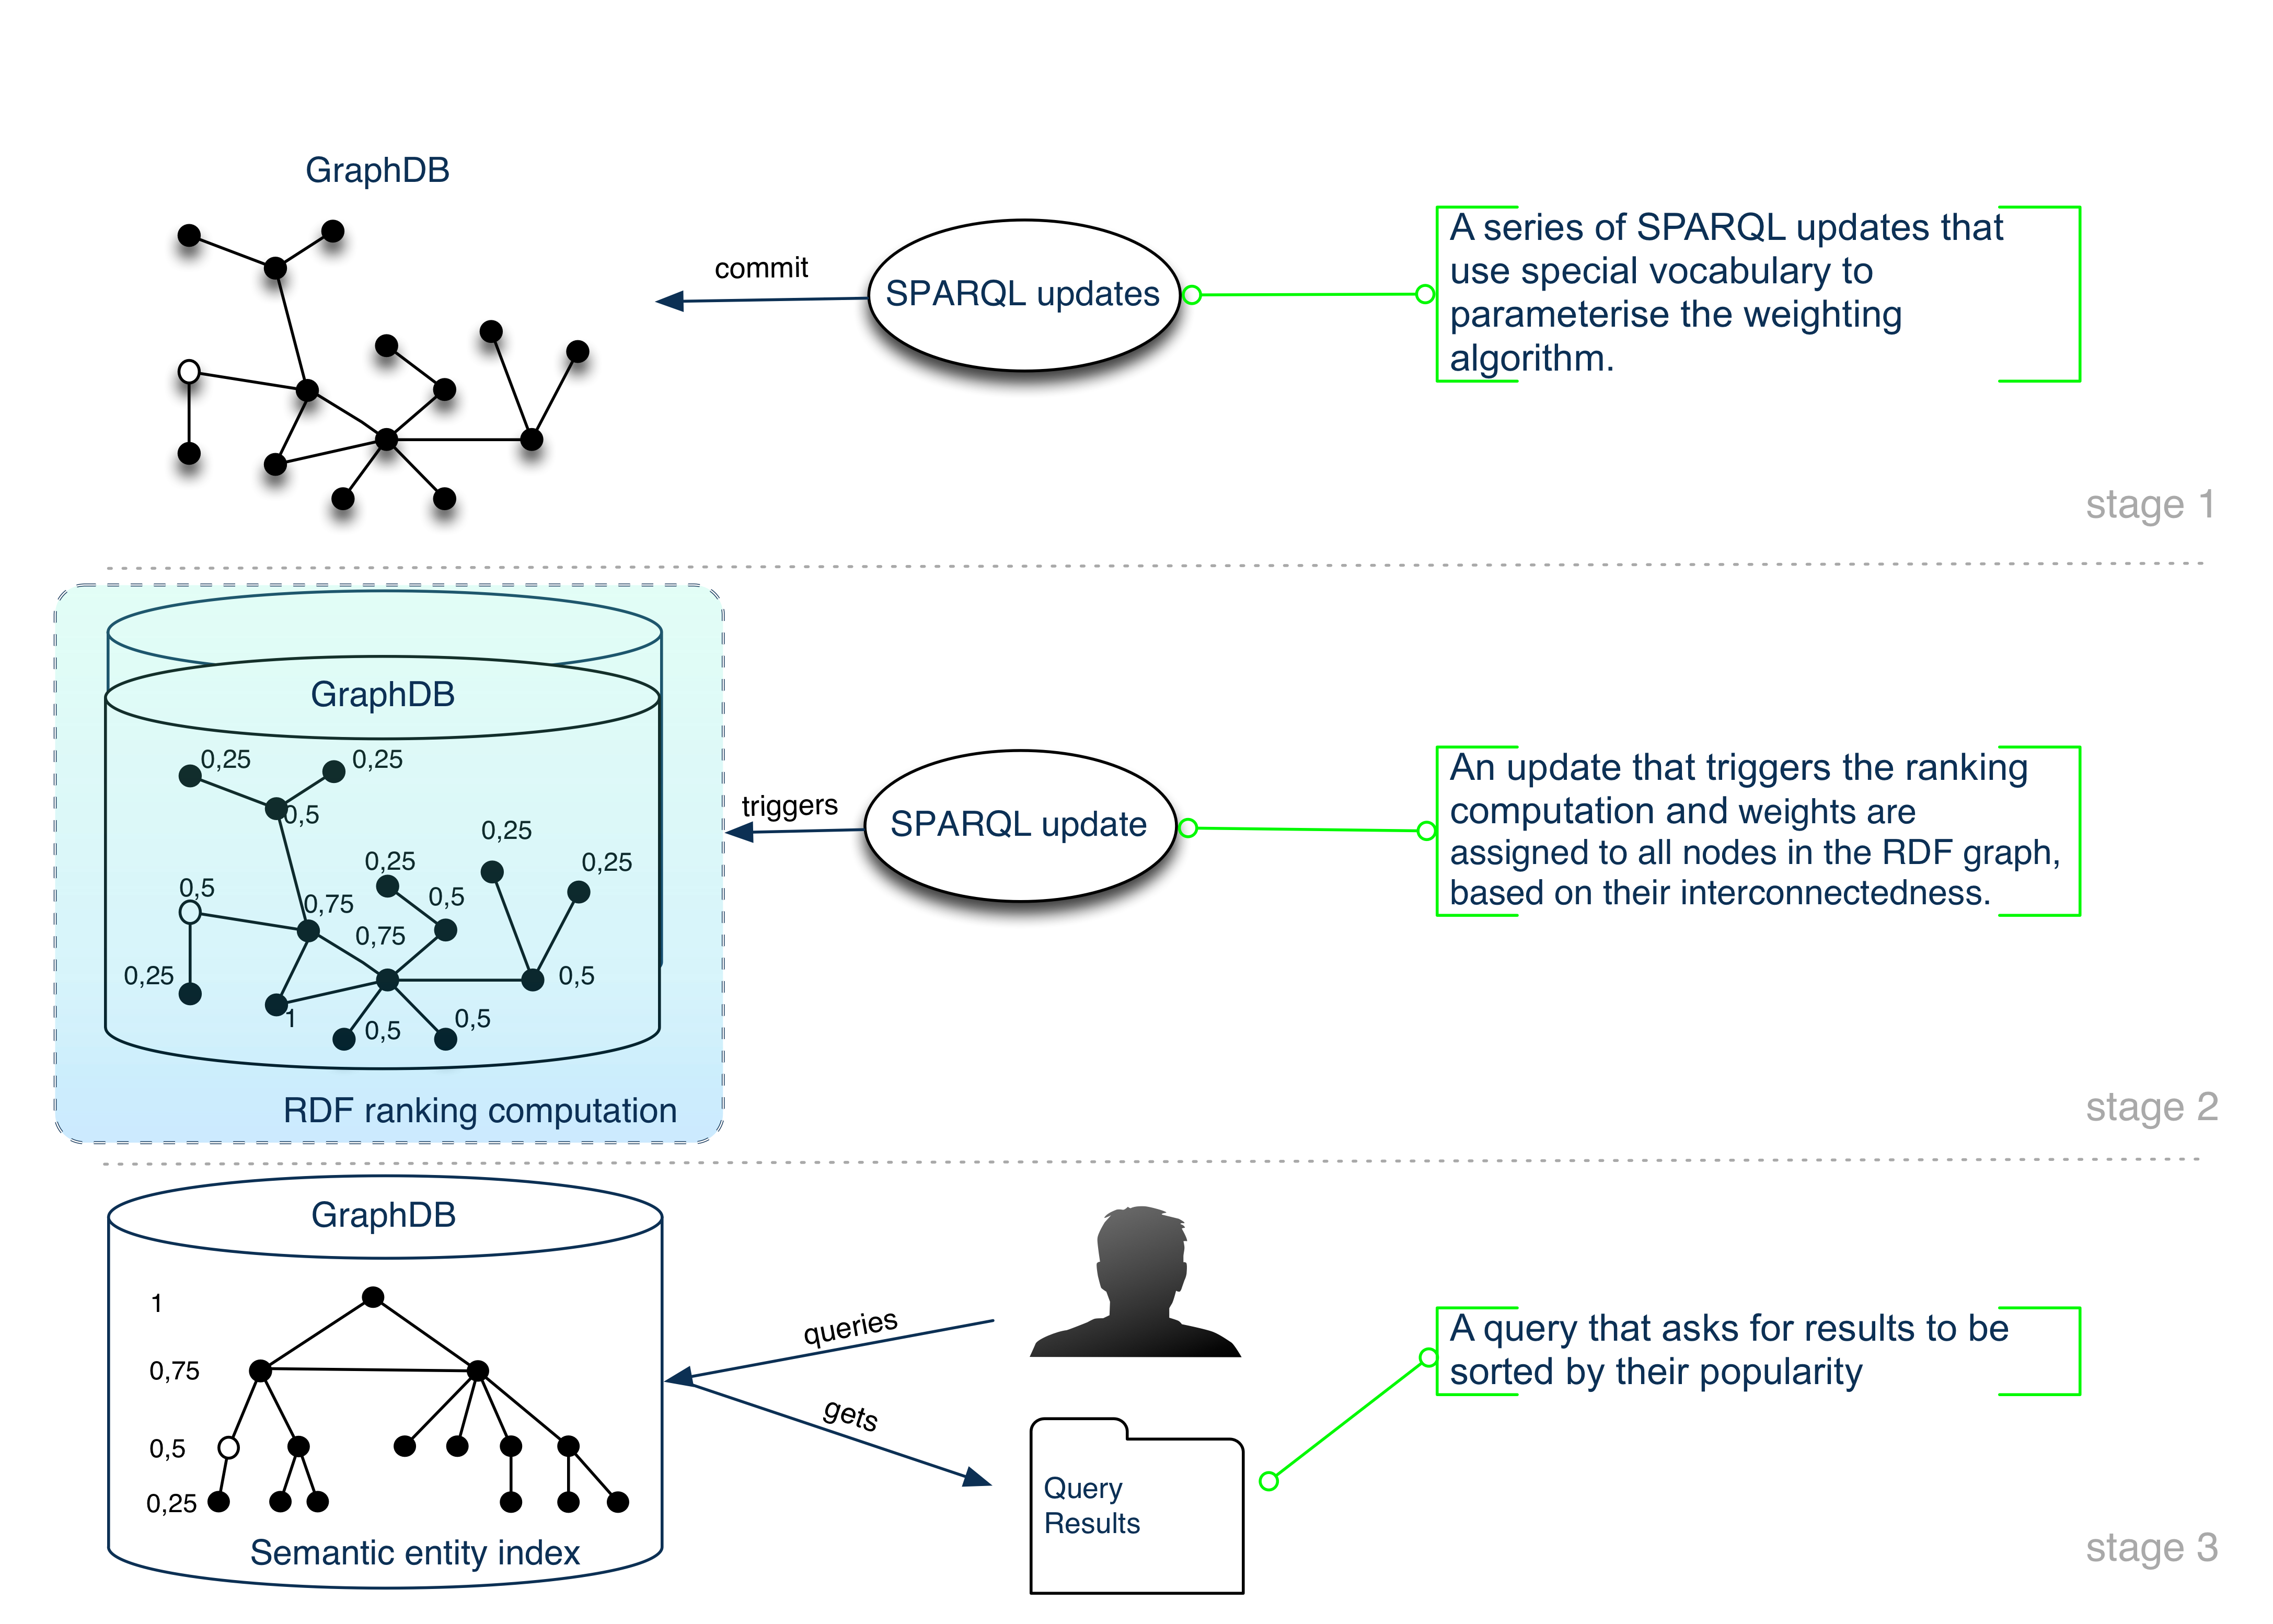
\includegraphics[width=\linewidth]{rdf-rank}
    \caption{RDF Rank plugin workflow}
    \label{rdf-rank}
\end{figure}

\textbf{Context indices} are another optimization that could be utilised, so they will be enabled. There are two types of context indices used to speed up query evaluation when searching statements via their context identifier. These indices are the PCSO (Predicate-Context-Subject-Object) and the PCOS (Predicate-Context-Object-Subject) and they are switched on together.

Finally the \textbf{Lucene Connector} will be used on some key entities from DBPedia and GeoNames and also on news data as a separate index - title, content, creation dates, etc. The Connectors provide synchronisation at the entity level, where an entity is defined as having a unique identifier (a URI) and a set of properties and property values. In terms of RDF, this corresponds to a set of triples that have the same subject. In addition to simple properties (defined by a single triple), the Connectors support property chains. A property chain is defined as a sequence of triples where each triple’s object is the subject of the following triple.

\subsection{FactForge News}
Ontotext has an old free service called \textit{FactForge}, found at \texttt{http://factforge.com}, which is something like a search engine for RDF data. It allows you to write SPARQL queries against these huge amounts of RDF data, e.g. you could ask \textit{"Which are all the airports that in 50km of range of my location?"}. It is basically a triplestore repository with imported and interlinked data sets like GeoNames, DBPedia, etc. and some custom mappings. The setup that has been described so far with our news data in this chapter resembles almost the same thing and eventually it will become exactly that. This huge repository filled with news and popular LOD data sets using the newest version of GraphDB\textsuperscript{TM} and a way more feature-rich and refined Workbench as the user interface, will replace the old FactForge service. It is now called \textit{FactForge News} due to the added news data that was missing in the old one. The next two figures give a small overview of the RDF classes and RDF domain and range relationships of a particular class:

\begin{figure}[h!]
    \centering
    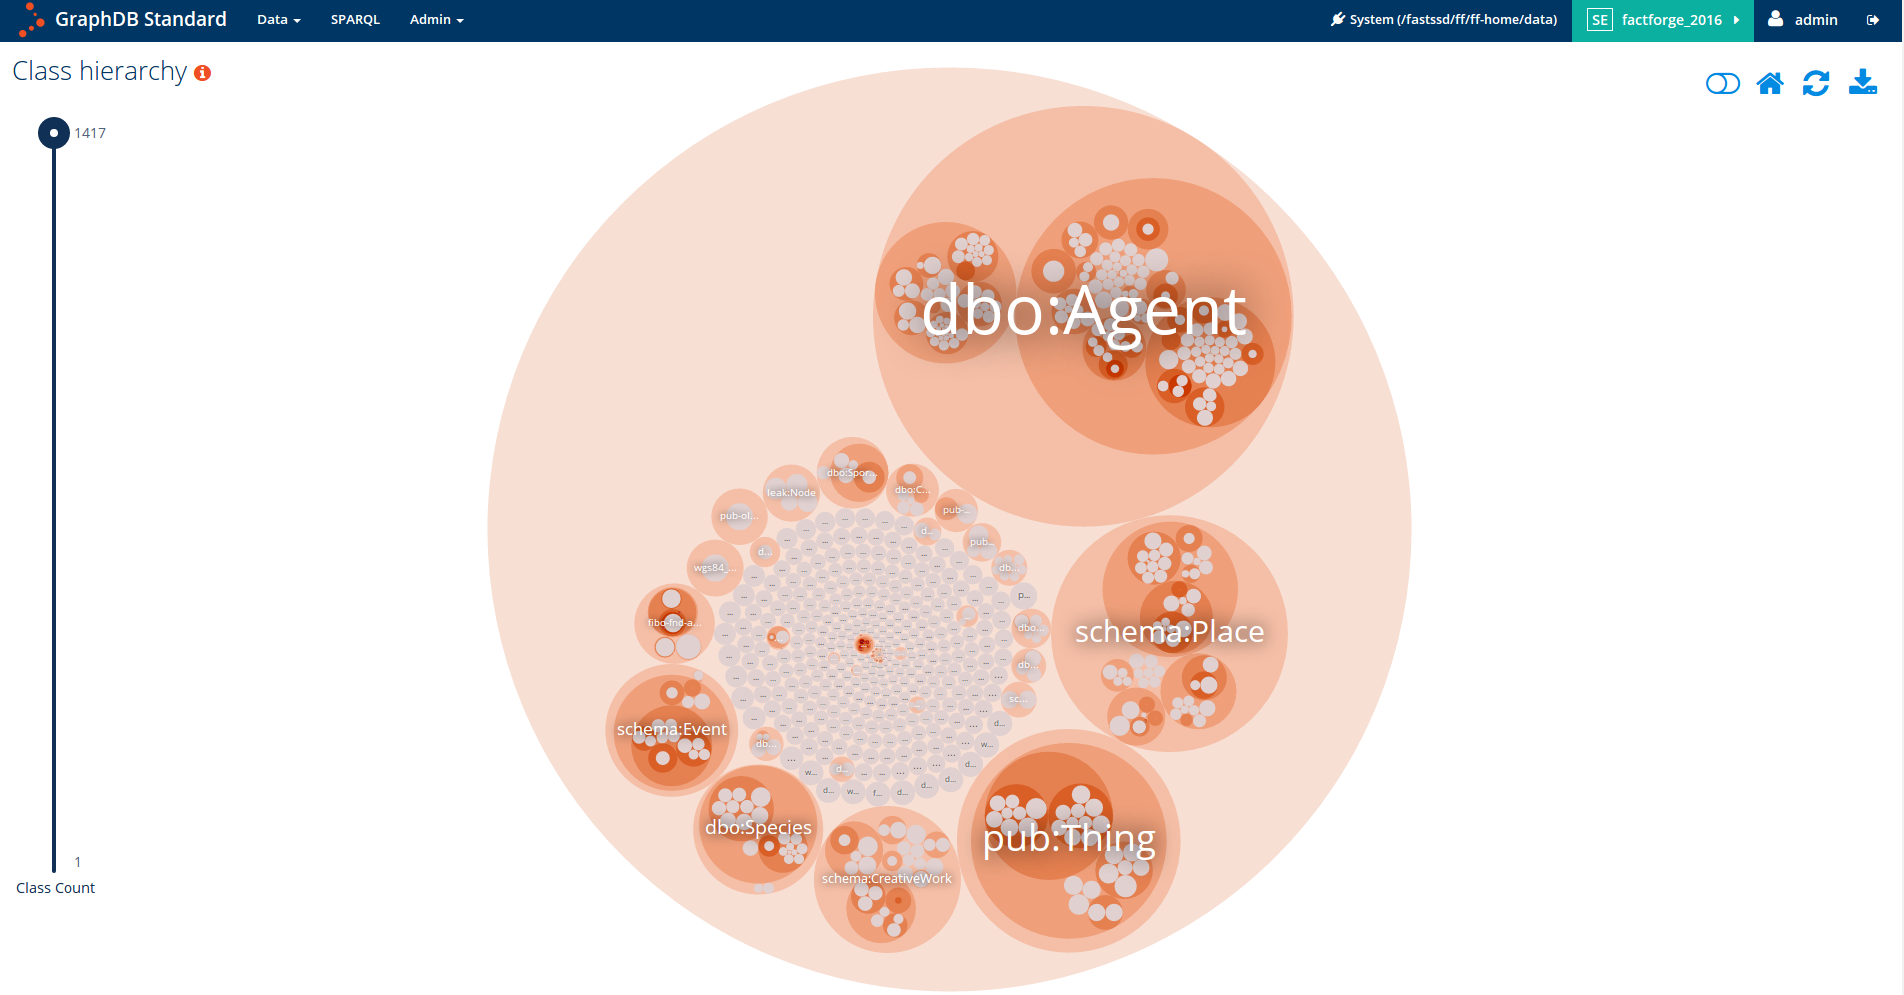
\includegraphics[width=\linewidth]{ff-news-hierarchy}
    \caption{Fact Forge News RDF class hierarchy diagram}
    \label{fig:ff-news-hierarchy}
\end{figure}

\begin{figure}[h!]
    \centering
    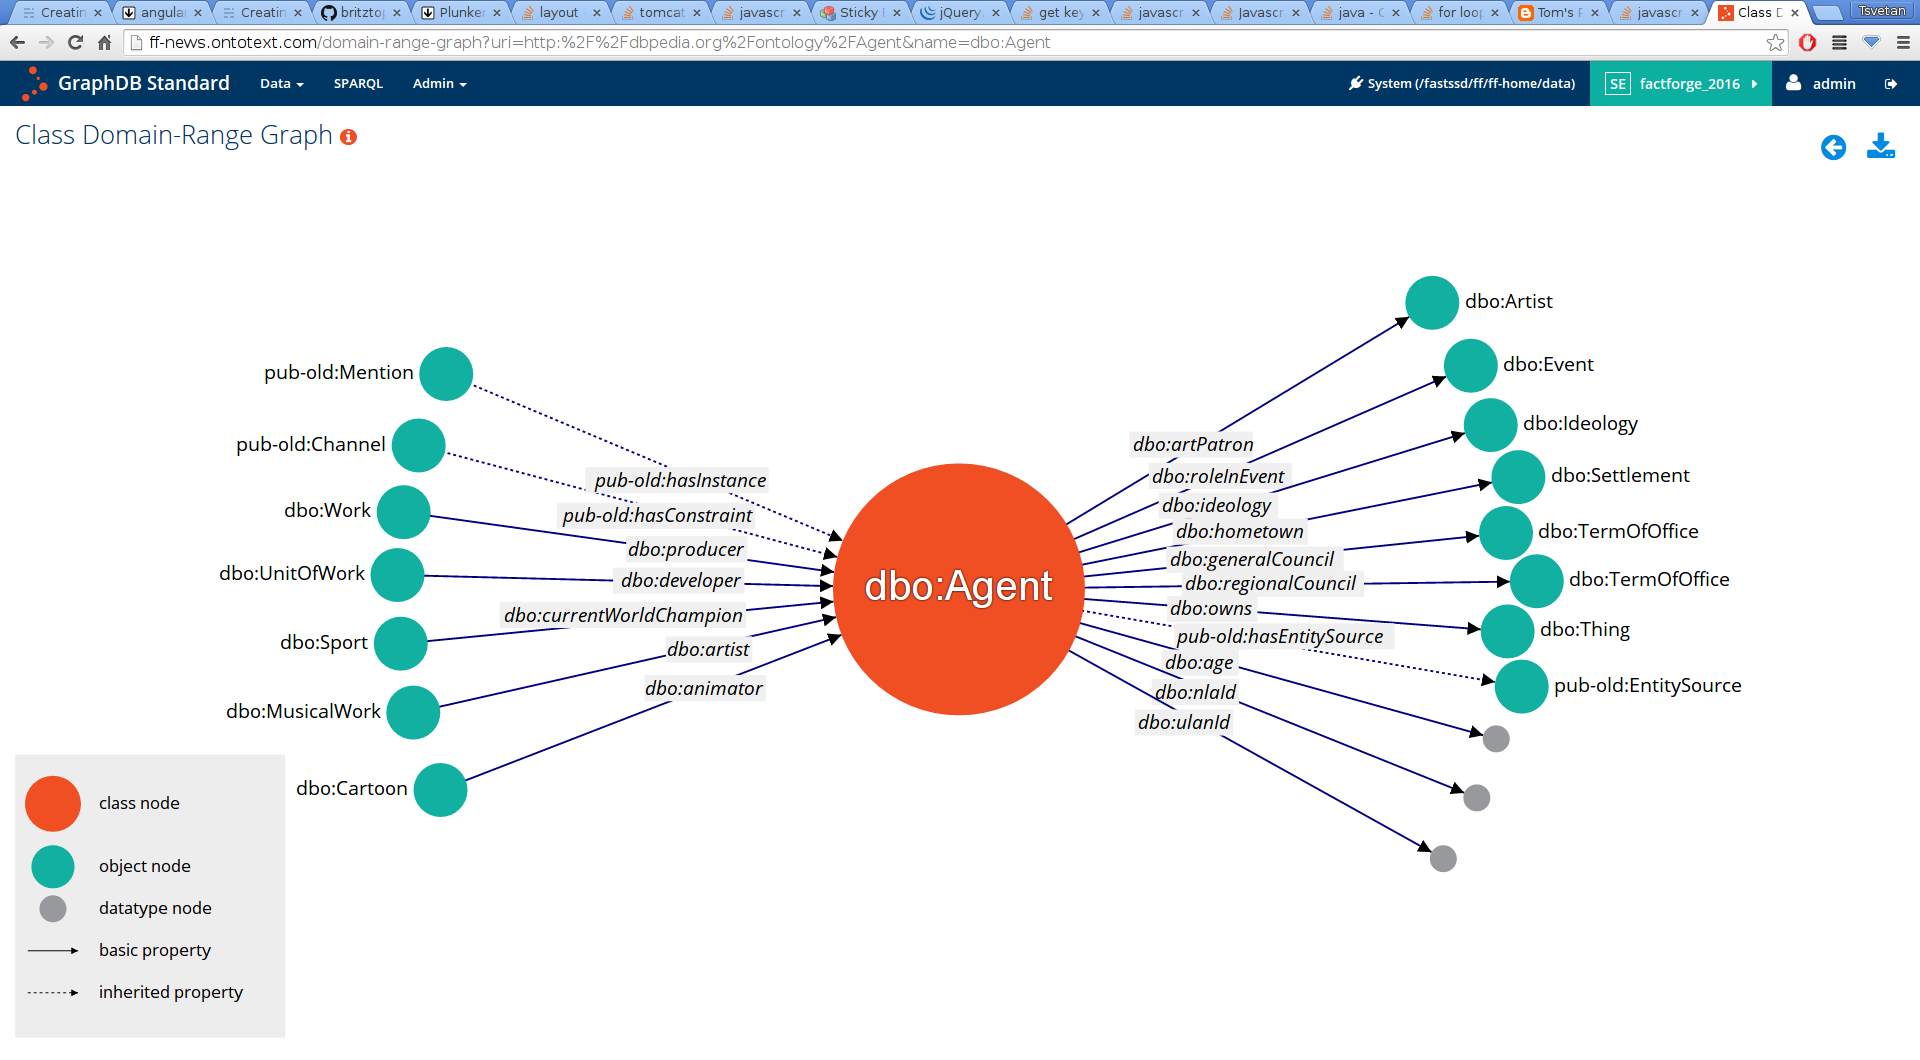
\includegraphics[width=\linewidth]{domain-range-graph-agent}
    \caption{Fact Forge News Agent RDF class domain-range graph diagram}
    \label{fig:domain-range-graph-agent}
\end{figure}
The \textit{Semantic News Map} application presented in \textit{Chapter \ref{chap:semnews-app}} will use \textit{FactForge News} as a data repository. 
